\section{Ejercicio 1}

El ejercio 1 consiste en realizar un producto vectorial sencillo, empleando distintos m\'etodos.
Se utiliz\'o la libreria thrust para las versiones en C++ de CPU y de GPU, y se uso PyCUDA para
la version en Python.

La soluci\'on para la libreria thrust es utilizar la funci\'on transform, que toma varios parametros
de entrada, donde se definen los operandos, el lugar de destino y el operador. En nuestro caso,
se aplic\'a transform de la siguiente manera:

\texttt{
    thrust::transform(D1.begin(), D1.end(), D2.begin(), D3.begin(),
                       thrust::multiplies<float>());
}

Esto se define como: Tomar los datos de D1, de comienzo a fin, combinarlo con el dato de D2 al aplicarle la funci\'on 
de \texttt{thrust::multiplies<float>()} y dejarlo en D3. Una ventaja de thrust es que es totalmente 
portable entre CPU y GPU. Otra ventaja es que es muy idiomatico de C++, no hay ninguna construcci\'on muy rara
que no se encastre en el lenguaje. 


  \begin{figure}[H]
 \begin {center}
 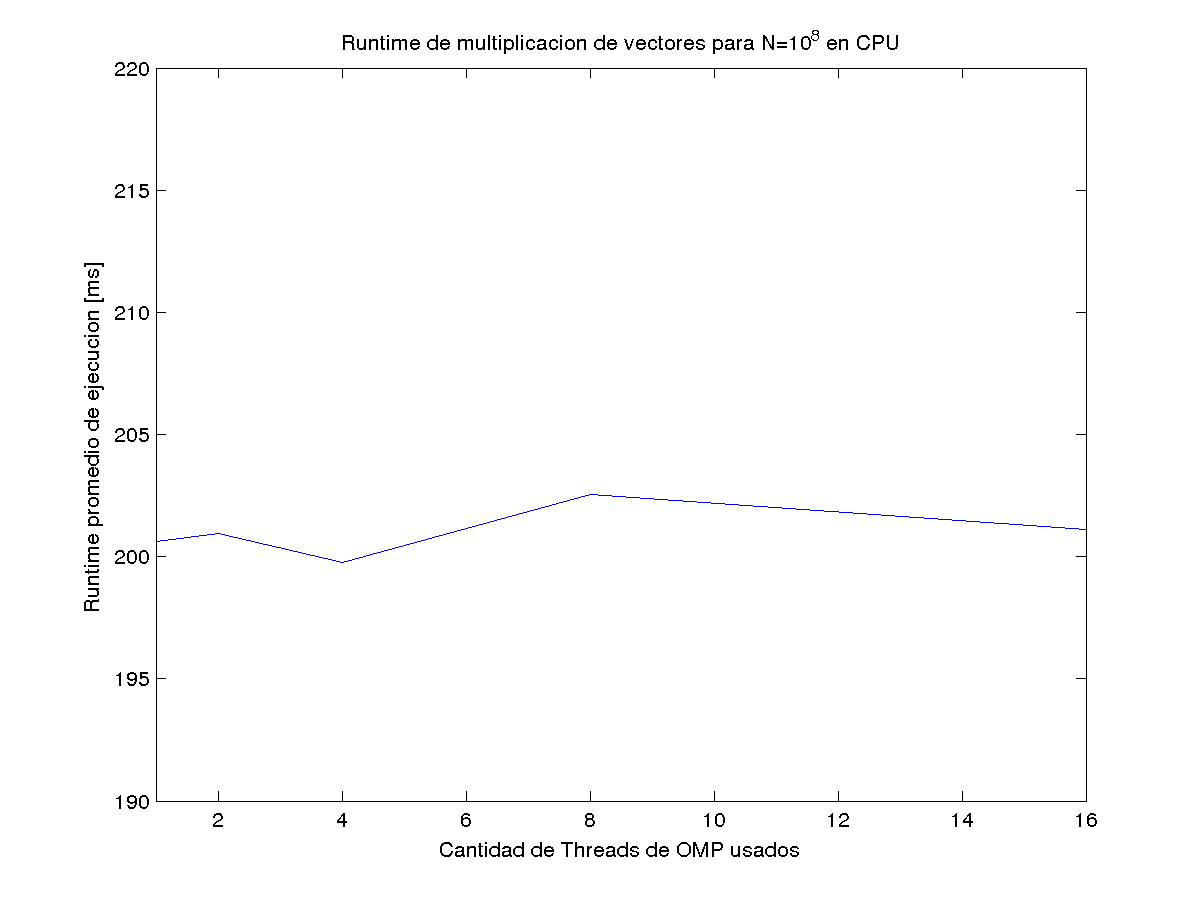
\includegraphics[width=\hrwidth]{plots/ej1omp.png}
 \end {center}
 \caption{Runtime del ej1 en Thrust con OMP, en funcion de la cantidad de threads, para una longitud de vectores $L=10^8$}
 \label{fig:ej1OMP}
 \end{figure}

\begin{table}
    \begin{tabular}{l|l}
        \textbf{M\'etodo} & \textbf{ Runtime [ms] }\\ \hline
    1 OMP Thread         & 200.598      \\
    2 OMP Thread          & 200.963      \\
    4 OMP Thread          & 199.766      \\
    8 OMP Thread  & 202.534      \\
    16 OMP Thread & 201.127      \\
        CUDA M2090 & 11.035 
    \end{tabular}
\end{table}



 Como se puede ver en el gr\'afico y la tabla de la figura \ref{fig:ej1OMP}, casi no varian los runtimes a pesar de tener
 muchos threads. Esto se debe a que el costo de generar y spawnear threads nuevos es tan alto que el procesador
 deberia hacer m\'as c\'alculo por core en vez de paralelizar m\'as el problema. Esto es un claro ejemplo
 de una tarea que es demasiado chica para threadear, e incluso con un problema relativamente grande de $10^8$ 
 elementos, no vale la pena paralelizarlo con CPU.

 Comparado contra la placa Nvidia con CUDA, podemos apreciar la diferencia de velocidad notablemente. Esto igual no toma
 en cuenta el tiempo de transferencia de memoria, por lo cual puede llegar a ser engañoso a veces el tiempo de runtime
 en las comparaciones CPU/GPU.
